\subsection{TPC-DS sharing}
\label{sec:tpcds-sharing}

We discuss the optimization opportunities and challenges through the following example of 3 queries (Query 3, 43 and 55) from the TPC-DS benchmark \cite{tpcds}:
\begingroup
\fontsize{6pt}{7pt}
\selectfont
\begin{verbatim}
Query 3:
SELECT d_year, i_brand_id, i_brand, sum(ss_ext_sales_price) AS sum_agg
FROM  date_dim, store_sales, item
WHERE d_date_sk = ss_sold_date_sk
AND ss_item_sk = i_item_sk
AND i_manufact_id = 128
AND d_moy=11
GROUP BY d_year, i_brand, i_brand_id
ORDER BY d_year, sum_agg desc, i_brand_id
LIMIT 100

Query 55:
SELECT i_brand_id, i_brand, 
sum(ss_ext_sales_price) ext_price
FROM date_dim, store_sales, item
WHERE d_date_sk = ss_sold_date_sk
AND ss_item_sk = i_item_sk
AND i_manager_id=28
AND d_moy=11
AND d_year=1999
GROUP BY i_brand, i_brand_id
ORDER BY ext_price desc, i_brand_id
LIMIT 100

Query 43:
SELECT s_store_name, s_store_id, 
sum(case when (d_day_name='Sunday') 
then ss_sales_price else null end) sun_sales,
sum(case when (d_day_name='Monday') 
then ss_sales_price else null end) mon_sales,
...
sum(case when (d_day_name='Saturday') 
then ss_sales_price else null end) sat_sales
FROM date_dim, store_sales, store
WHERE d_date_sk = ss_sold_date_sk 
AND s_store_sk = ss_store_sk
AND s_gmt_offset = -5
AND d_year = 2000
GROUP BY s_store_name, s_store_id
ORDER BY s_store_name, s_store_id,sun_sales,mon_sales,tue_sales,
wed_sales, thu_sales,fri_sales,sat_sales
LIMIT 100
\end{verbatim}
\endgroup

\begin{figure*}[htbp]
	\centering
	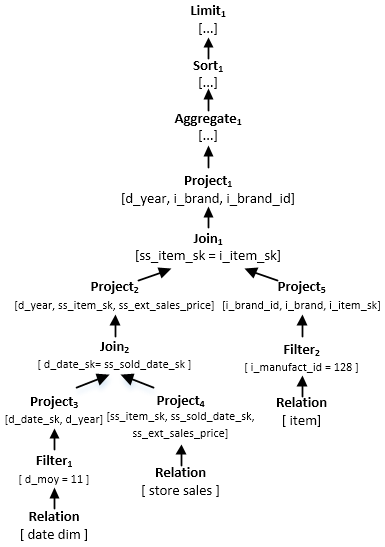
\includegraphics[scale=0.5]{figures/q3}
	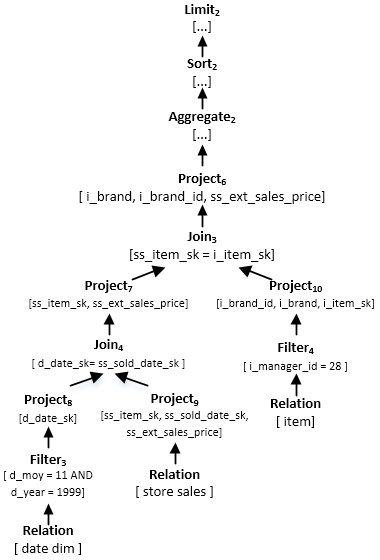
\includegraphics[scale=0.5]{figures/q55}
	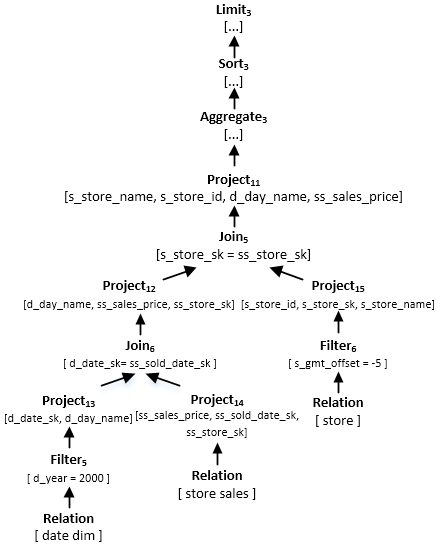
\includegraphics[scale=0.5]{figures/q43}
	\caption{Optimized operator trees of query 3, 55 and 43 (from left to right) in the TPC-DS benchmark} 
	\label{fig:queries}
\end{figure*}